\section{Proof of Proposition~\ref{prop:bb}}
\label{app:proof}

\emph{Exchangeable case.} Because the $n+m$ scores are exchangeable and almost surely distinct, the ordering of the scores by value is a uniformly random arrangement of $n$ calibration and $m$ audit labels. Sort all scores in decreasing order. The threshold $\hat\tau=S_{(k)}$ is the $(n-k+1)$-th calibration score from the top, so exactly $a-1=n-k$ calibration scores lie above it. The event $\{X=x\}$ occurs when the first $x+n-k$ positions hold $x$ audit and $n-k$ calibration scores, the next position holds $\hat\tau$, and the remaining $m-x+k-1$ positions hold $m-x$ audit and $k-1$ calibration scores. Hence
\[
P(X=x)=\frac{\binom{x+a-1}{x}\binom{m-x+b-1}{m-x}}{\binom{n+m}{m}},\qquad x=0,\dots,m,
\]
with $a=n+1-k$ and $b=k$. This is the Beta-Binomial$(m,a,b)$ probability mass function, by the standard negative-hypergeometric (P\'olya urn) identity. We also checked the identity numerically to machine precision for all $(n,k,m)$ used in this paper. Its mean is $ma/(a+b)=ma/(n+1)$.

\emph{I.i.d.\ continuous case.} Let $G$ be the continuous distribution function of authentic scores and $U_i=G(S_i)$, which are i.i.d.\ uniform. Then $G(\hat\tau)=U_{(k)}\sim\mathrm{Beta}(k,n+1-k)$ and $\mathrm{FPR}(\hat\tau)=1-G(\hat\tau)\sim\mathrm{Beta}(n+1-k,k)$ \citep{vovk2012conditional}. Given the calibration set, the $m$ audit indicators $\mathbb{1}[S_j>\hat\tau]$ are i.i.d.\ Bernoulli$(\mathrm{FPR})$, so $X\mid\mathrm{FPR}\sim\mathrm{Binomial}(m,\mathrm{FPR})$, and mixing over the Beta law gives the same Beta-Binomial distribution. \Eqref{eq:pviol} is its upper tail. \qed

\emph{Ties.} If scores can tie and alerts require $s>\hat\tau$, breaking ties at random gives a version with distinct scores in which $X$ can only be larger, so $X$ is stochastically dominated by the Beta-Binomial law and the rule is conservative.

\section{Pre-registration and deviations}
\label{app:prereg}

Hypotheses, decision rules, dataset roles and analysis code paths were recorded in an append-only decision log in the code repository before the corresponding analyses. Confirmatory data were frozen by committing manifests and tagging the commit (\texttt{prereg-freeze-h7} for the FakeAVCeleb manifest, \texttt{prereg-freeze-h8} for the H8 design); FakeAVCeleb score files were hashed and committed before they were opened. The log, tags and hashes are in the supplementary material. Table~\ref{tab:dev} lists every logged deviation that affects a reported result.

\begin{table}[h]
\centering
\small
\caption{Logged deviations from the registered plan and how they are handled in this paper.}
\label{tab:dev}
\begin{tabular}{l p{6.2cm} p{6.0cm}}
\toprule
ID & Deviation & Handling here \\
\midrule
D1, D19 & Five training seeds per model registered; three trained & H1 and H4a reported as undetermined; three-seed results descriptive \\
D2, D3 & Early H1 runs used too few resamples, unadjusted intervals and the wrong comparison pairs & Re-run with 10{,}000 resamples, Bonferroni, ST--S and Full--S \\
D4, D14 & DFD negatives initially included FF++ reals & Only the 243 DFD actor reals are used \\
D5, D13 & H2 threshold applied on the wrong scale; coarse bootstrap clusters & Calibrated scale, identity clusters; H2 undetermined \\
D6 & H3a posteriors uncalibrated; HTER is prior-invariant & Calibrated posteriors, all runs; H3a kept as registered (falsified) \\
D7 & Comparison to GenD made before the official checkpoint was run & Official checkpoint run through the same pipeline \\
D8 & DFD overlaps development data & DFD is development data only \\
D10 & FPR bootstrap used coarse clusters & Identity-level clusters \\
D11 & Seeds seen before registration counted as confirmatory for H4 & Excluded; H4a undetermined \\
D12 & Out-of-support mixture thresholds not flagged & Flagged as degenerate \\
D15 & An ablation changed only part of the readout & Not used for any claim \\
D16 & Two definitions of TPR at $5\%$ FPR & One conservative definition throughout \\
D17 & Trainable parameters of S-MSDT-S misreported & Counts built from training configurations; S and GenD-style not footprint-matched \\
D18 & Celeb-DF reals mix two sources; video- vs identity-weighted FPR & Both weights reported; H7b-v2 requires both; per-source results exploratory \\
D20 & H8 registered after H7 & Reported as registered; verdict falsified \\
\bottomrule
\end{tabular}
\end{table}

\paragraph{H7 revision.} The first version of H7 compared shape-transfer estimators fitted to 10 and 20 target reals. On the Celeb-DF and DFD development data its two main conditions were not supported for most detectors. It was then revised to the version reported here (H7a--c-v2) before FakeAVCeleb was scored. We report both versions. On FakeAVCeleb the first version remains not supported: its H7a condition fails for every detector family and its H7b condition for two of the five.

\section{Detector and training details}
\label{app:models}

\paragraph{Backbone.} CLIP ViT-L/14 at $224\times224$ input, patch size 14, width 1024. All weights are frozen except the LayerNorm scale and shift parameters ($102{,}400$).

\paragraph{Heads.} GenD-style (ours) uses an L2-normalized class token and a linear classifier ($1{,}025$ head parameters). S-MSDT-S projects patch tokens to width 384 and pools them with an attention-based multiple-instance readout and a class-token head ($675{,}078$). S-MSDT-ST adds learned temporal position embeddings and two transformer blocks whose queries also receive temporal differences $\Delta Z_t=Z_t-Z_{t-1}$, with a top-$k$ readout. S-MSDT-Full adds a residual stream: three fixed $5\times5$ SRM high-pass filters \citep{fridrich2012rich} and the high-frequency sub-bands of a two-level Haar wavelet transform are projected to the token width and added to the patch tokens through a learned sigmoid gate initialized at $\sigma(-4)\approx0.018$; its readout uses four learned queries, an additive bias towards a mouth-region mask derived from facial landmarks, and log-sum-exp pooling with a learned temperature (initial value 3).

\paragraph{Training.} FaceForensics++ c23 training split, five manipulation methods with matched real--fake pairs; 30 epochs; 16 pairs per step; learning rates $10^{-4}$ for LayerNorm and $5\times10^{-4}$ for the head, $3\%$ warm-up and decay to $1\%$ of the peak rate; weight decay $0.05$; label smoothing $0.05$; gradient clipping at $1$; an exponential moving average of weights (decay $0.999$) selected on FF++ validation from epoch 5; seeds 1--3. The published GenD checkpoint is used as released.

\paragraph{Compute.} Each video is scored from 8 clips; temporal models process 64 frames per video and single-frame models 8.

\section{Additional results}
\label{app:extra}

% AUTO-GENERATED by tools/paper_tables.py -- do not edit by hand
\begin{table}[h]
\centering
\scriptsize
\setlength{\tabcolsep}{3pt}
\caption{Per-run results. TPR5 is the TPR at the conservative empirical $5\%$-FPR point on each test set.}
\label{tab:appx_per_run}
\begin{tabular}{l c c c cc cc cc cc}
\toprule
 & & & & \multicolumn{2}{c}{FF++ (test)} & \multicolumn{2}{c}{Celeb-DF} & \multicolumn{2}{c}{DFD} & \multicolumn{2}{c}{FakeAVCeleb}\\
\cmidrule(lr){5-6}\cmidrule(lr){7-8}\cmidrule(lr){9-10}\cmidrule(lr){11-12}
Detector & Seed & Trainable & $T$ & AUC & TPR5 & AUC & TPR5 & AUC & TPR5 & AUC & TPR5 \\
\midrule
GenD (official)$^\dagger$ & 0 & 0.10M & 1 & 0.945 & 0.847 & 0.933 & 0.738 & 0.884 & 0.650 & 0.974 & 0.906 \\
GenD-style (ours) & 1 & 0.10M & 1 & 0.905 & 0.727 & 0.832 & 0.521 & 0.866 & 0.699 & 0.890 & 0.649 \\
GenD-style (ours) & 2 & 0.10M & 1 & 0.904 & 0.726 & 0.827 & 0.512 & 0.869 & 0.710 & 0.890 & 0.643 \\
GenD-style (ours) & 3 & 0.10M & 1 & 0.904 & 0.733 & 0.829 & 0.515 & 0.862 & 0.702 & 0.893 & 0.651 \\
S-MSDT-S & 1 & 0.78M & 1 & 0.959 & 0.841 & 0.884 & 0.503 & 0.867 & 0.651 & 0.947 & 0.826 \\
S-MSDT-S & 2 & 0.78M & 1 & 0.961 & 0.857 & 0.883 & 0.506 & 0.878 & 0.692 & 0.944 & 0.822 \\
S-MSDT-S & 3 & 0.78M & 1 & 0.968 & 0.867 & 0.882 & 0.515 & 0.888 & 0.684 & 0.940 & 0.798 \\
S-MSDT-ST & 1 & 8.47M & 8 & 0.960 & 0.854 & 0.871 & 0.453 & 0.861 & 0.588 & 0.932 & 0.774 \\
S-MSDT-ST & 2 & 8.47M & 8 & 0.966 & 0.870 & 0.878 & 0.421 & 0.856 & 0.576 & 0.948 & 0.817 \\
S-MSDT-ST & 3 & 8.47M & 8 & 0.962 & 0.863 & 0.863 & 0.544 & 0.870 & 0.656 & 0.937 & 0.799 \\
S-MSDT-Full & 1 & 9.10M & 8 & 0.963 & 0.884 & 0.891 & 0.518 & 0.832 & 0.465 & 0.946 & 0.799 \\
S-MSDT-Full & 2 & 9.10M & 8 & 0.962 & 0.849 & 0.896 & 0.550 & 0.858 & 0.563 & 0.944 & 0.790 \\
S-MSDT-Full & 3 & 9.10M & 8 & 0.962 & 0.879 & 0.877 & 0.509 & 0.844 & 0.520 & 0.945 & 0.802 \\
\bottomrule
\end{tabular}
\end{table}

% AUTO-GENERATED by tools/paper_tables.py -- do not edit by hand
\begin{table}[h]
\centering
\small
\caption{Per-run real-shot results on FakeAVCeleb at $n=20$, $\alpha=0.05$ (500 draws).}
\label{tab:appx_real_shot_runs}
\begin{tabular}{lc ccccc cc}
\toprule
 & & \multicolumn{5}{c}{Conformal} & \multicolumn{2}{c}{Naive quantile}\\
\cmidrule(lr){3-7}\cmidrule(lr){8-9}
Detector & Seed & FPR & $P(>2\alpha)$ & TPR & Oracle TPR & Retained & FPR & $P(>2\alpha)$ \\
\midrule
GenD (official)$^\dagger$ & 0 & 0.0459 & 0.114 & 0.849 & 0.917 & 92.7\% & 0.0897 & 0.376 \\
GenD-style (ours) & 1 & 0.0455 & 0.092 & 0.546 & 0.652 & 83.8\% & 0.0861 & 0.328 \\
GenD-style (ours) & 2 & 0.0450 & 0.096 & 0.538 & 0.644 & 83.5\% & 0.0867 & 0.306 \\
GenD-style (ours) & 3 & 0.0454 & 0.100 & 0.556 & 0.653 & 85.2\% & 0.0855 & 0.320 \\
S-MSDT-S & 1 & 0.0449 & 0.104 & 0.797 & 0.836 & 95.4\% & 0.0884 & 0.350 \\
S-MSDT-S & 2 & 0.0472 & 0.130 & 0.799 & 0.825 & 96.8\% & 0.0888 & 0.370 \\
S-MSDT-S & 3 & 0.0471 & 0.130 & 0.779 & 0.805 & 96.8\% & 0.0872 & 0.370 \\
S-MSDT-ST & 1 & 0.0462 & 0.120 & 0.737 & 0.785 & 93.8\% & 0.0897 & 0.320 \\
S-MSDT-ST & 2 & 0.0469 & 0.112 & 0.770 & 0.826 & 93.3\% & 0.0897 & 0.394 \\
S-MSDT-ST & 3 & 0.0462 & 0.132 & 0.750 & 0.798 & 94.0\% & 0.0850 & 0.326 \\
S-MSDT-Full & 1 & 0.0439 & 0.108 & 0.745 & 0.808 & 92.2\% & 0.0871 & 0.352 \\
S-MSDT-Full & 2 & 0.0441 & 0.118 & 0.738 & 0.776 & 95.0\% & 0.0872 & 0.350 \\
S-MSDT-Full & 3 & 0.0453 & 0.106 & 0.772 & 0.812 & 95.1\% & 0.0869 & 0.382 \\
\bottomrule
\end{tabular}
\end{table}

% AUTO-GENERATED by tools/paper_tables.py -- do not edit by hand
\begin{table}[h]
\centering
\small
\caption{The six H8 cells that fail validity criterion (ii). All are on FakeAVCeleb. $z$ is the excess of the mean FPR over $\alpha$ in Monte Carlo standard errors.}
\label{tab:appx_h8_fail}
\begin{tabular}{lc cc cccc}
\toprule
Detector & Seed & $\alpha$ & $n$ & Mean FPR & Excess & $\mathrm{SE}_{\mathrm{MC}}$ & $z$ \\
\midrule
S-MSDT-S & 1 & 0.05 & 19 & 0.0532 & 0.0032 & 0.0016 & 2.05 \\
S-MSDT-S & 1 & 0.05 & 59 & 0.0527 & 0.0027 & 0.0010 & 2.67 \\
S-MSDT-ST & 1 & 0.05 & 19 & 0.0531 & 0.0031 & 0.0016 & 2.01 \\
S-MSDT-ST & 1 & 0.05 & 59 & 0.0520 & 0.0020 & 0.0010 & 2.01 \\
S-MSDT-ST & 2 & 0.10 & 9 & 0.1062 & 0.0062 & 0.0030 & 2.07 \\
S-MSDT-ST & 2 & 0.10 & 29 & 0.1037 & 0.0037 & 0.0017 & 2.10 \\
\bottomrule
\end{tabular}
\end{table}

% AUTO-GENERATED by tools/paper_tables.py -- do not edit by hand
\begin{table}[h]
\centering
\small
\caption{Post-hoc check (not registered): the H8 evaluation re-run with different random seeds. Mean $z$ is the average standardized excess $(\overline{\mathrm{FPR}}-\alpha)/\mathrm{SE}_{\mathrm{MC}}$ over the 65 cells of a target; ``fail'' counts cells violating criterion (ii). Under an exact law about $3$ of $130$ cells are expected to fail.}
\label{tab:appx_h8_reseed}
\begin{tabular}{l cc cc c}
\toprule
 & \multicolumn{2}{c}{FakeAVCeleb} & \multicolumn{2}{c}{Celeb-DF} & \\
\cmidrule(lr){2-3}\cmidrule(lr){4-5}
Seed & mean $z$ & fail & mean $z$ & fail & Total fail \\
\midrule
42 (registered) & +0.63 & 6 & -0.22 & 0 & 6/130 \\
101 & -0.22 & 1 & -0.83 & 0 & 1/130 \\
202 & -0.30 & 0 & -0.25 & 3 & 3/130 \\
303 & -0.43 & 3 & +0.04 & 0 & 3/130 \\
\bottomrule
\end{tabular}
\end{table}

% AUTO-GENERATED by tools/paper_tables.py -- do not edit by hand
\begin{table}[h]
\centering
\small
\caption{Celeb-DF development split, conformal calibration within each source of authentic video ($\alpha=0.05$), mean over the 13 detectors. Exploratory; the YouTube stratum is small.}
\label{tab:appx_strata}
\begin{tabular}{l c c ccc}
\toprule
Real stratum & $n$ & Identities & Mean FPR & $P(\mathrm{FPR}>2\alpha)$ & TPR \\
\midrule
Celeb-real & 20 & 51 & 0.045 & 0.123 & 0.469 \\
YouTube-real & 20 & 70 & 0.048 & 0.123 & 0.466 \\
\bottomrule
\end{tabular}
\end{table}

% AUTO-GENERATED by tools/paper_tables.py -- do not edit by hand
\begin{table}[h]
\centering
\small
\setlength{\tabcolsep}{3.5pt}
\caption{Test-time adaptation of LayerNorm parameters (S-MSDT-Full, seed 1, learning rate $10^{-4}$). ``Collapsed'' follows the pre-registered rule: AUC drop $>0.03$, or predicted-positive share outside $[5\%,95\%]$.}
\label{tab:appx_tta}
\begin{tabular}{lll ccc cc c}
\toprule
Target & Objective & Mode & Pre AUC & Post AUC & $\Delta$ & Pred.\ pos. & True pos. & Collapsed \\
\midrule
Celeb-DF-v2 & entropy & online & 0.8880 & 0.3386 & -0.5494 & 6.6\% & 65.6\% & yes \\
Celeb-DF-v2 & entropy & batch-episodic & 0.8880 & 0.8880 & +0.0000 & 61.0\% & 65.6\% & no \\
DFD & entropy & online & 0.8583 & 0.2390 & -0.6193 & 0.6\% & 87.2\% & yes \\
DFD & entropy & batch-episodic & 0.8583 & 0.8583 & +0.0000 & 70.7\% & 87.2\% & no \\
Celeb-DF-v2 & consistency & online & 0.8880 & 0.5409 & -0.3472 & 10.8\% & 65.6\% & yes \\
Celeb-DF-v2 & consistency & batch-episodic & 0.8880 & 0.8877 & -0.0003 & 60.4\% & 65.6\% & no \\
\bottomrule
\end{tabular}
\end{table}

% AUTO-GENERATED by tools/paper_tables.py -- do not edit by hand
\begin{table}[h]
\centering
\small
\caption{Prior-shift sweep on Celeb-DF with Saerens EM \citep{saerens2002adjusting}, averaged over all 13 detectors (calibrated posteriors). Exploratory.}
\label{tab:appx_prior}
\begin{tabular}{c c cc cc}
\toprule
Fake prior $\pi$ & $|\hat\pi-\pi|$ & HTER frozen & HTER after EM & Acc.\ frozen & Acc.\ EM-Bayes\\
\midrule
0.1 & 0.066 & 0.235 & 0.397 & 0.831 & 0.907 \\
0.3 & 0.110 & 0.228 & 0.284 & 0.802 & 0.808 \\
0.5 & 0.147 & 0.235 & 0.256 & 0.765 & 0.744 \\
0.7 & 0.165 & 0.234 & 0.249 & 0.734 & 0.745 \\
0.9 & 0.164 & 0.234 & 0.276 & 0.702 & 0.809 \\
\bottomrule
\end{tabular}
\end{table}

% AUTO-GENERATED by tools/paper_tables.py -- do not edit by hand
\begin{table}[h]
\centering
\small
\caption{Threshold transfer (H2). $g=\mathrm{HTER}(\tau_{\mathrm{val}})-\min_\tau\mathrm{HTER}(\tau)$ with the FF++-validation cutoff applied on the calibrated scale. The pre-registered H2 rule returns \emph{undetermined} for both reference detectors, so we draw no confirmatory conclusion from it.}
\label{tab:appx_h2}
\begin{tabular}{ll cc cc}
\toprule
Target & Detector & mean $g$ & max $g$ & FPR$(\tau_{\mathrm{val}})$ & FNR$(\tau_{\mathrm{val}})$\\
\midrule
Celeb-DF & GenD (official)$^\dagger$ & 0.021 & 0.021 & 0.213 & 0.115 \\
Celeb-DF & GenD-style (ours) & 0.017 & 0.026 & 0.266 & 0.252 \\
Celeb-DF & S-MSDT-S & 0.054 & 0.098 & 0.062 & 0.411 \\
Celeb-DF & S-MSDT-ST & 0.053 & 0.093 & 0.114 & 0.385 \\
Celeb-DF & S-MSDT-Full & 0.019 & 0.030 & 0.148 & 0.275 \\
\midrule
DFD & GenD (official)$^\dagger$ & 0.024 & 0.024 & 0.206 & 0.192 \\
DFD & GenD-style (ours) & 0.082 & 0.111 & 0.324 & 0.181 \\
DFD & S-MSDT-S & 0.009 & 0.015 & 0.063 & 0.311 \\
DFD & S-MSDT-ST & 0.020 & 0.036 & 0.144 & 0.299 \\
DFD & S-MSDT-Full & 0.010 & 0.012 & 0.166 & 0.308 \\
\bottomrule
\end{tabular}
\end{table}

% AUTO-GENERATED by tools/paper_tables.py -- do not edit by hand
\begin{table}[h]
\centering
\small
\caption{Corruption robustness on Celeb-DF (S-MSDT-Full, seed 1). Drop is clean AUC minus corrupted AUC.}
\label{tab:appx_robust}
\begin{tabular}{llcc}
\toprule
Corruption & Level & AUC & Drop \\
\midrule
Clean Baseline & None & 0.8884 & +0.0000 \\
JPEG Quality & 90 & 0.8972 & -0.0088 \\
JPEG Quality & 70 & 0.8829 & +0.0055 \\
JPEG Quality & 50 & 0.8482 & +0.0402 \\
JPEG Quality & 30 & 0.8048 & +0.0836 \\
Gaussian Blur (sigma) & 0.5 & 0.8920 & -0.0035 \\
Gaussian Blur (sigma) & 1.0 & 0.8732 & +0.0152 \\
Gaussian Blur (sigma) & 2.0 & 0.7987 & +0.0898 \\
Downscale Factor & 0.75 & 0.8907 & -0.0023 \\
Downscale Factor & 0.5 & 0.8734 & +0.0151 \\
Downscale Factor & 0.25 & 0.8217 & +0.0667 \\
\bottomrule
\end{tabular}
\end{table}

% AUTO-GENERATED by tools/paper_tables.py -- do not edit by hand
{\footnotesize\setlength{\tabcolsep}{3pt}
\begin{longtable}{l l c c c l}
\caption{All paired cluster-bootstrap comparisons. Only the two FakeAVCeleb rows marked confirmatory in Table~\ref{tab:h1} decide H1.}\label{tab:appx_h1}\\
\toprule
Dataset & Comparison & $\Delta$AUC & Interval & Level & Decision \\
\midrule
\endfirsthead
\toprule
Dataset & Comparison & $\Delta$AUC & Interval & Level & Decision \\
\midrule
\endhead
Celeb-DF & S-MSDT-ST $-$ S-MSDT-S & -0.0122 & [-0.0290, +0.0045] & 0.950 & inconclusive \\
DFD & S-MSDT-ST $-$ S-MSDT-S & -0.0151 & [-0.0254, -0.0047] & 0.950 & inconclusive \\
FakeAVCeleb & S-MSDT-ST $-$ S-MSDT-S & -0.0045 & [-0.0096, +0.0006] & 0.975 & equivalent \\
FF++ & S-MSDT-ST $-$ S-MSDT-S & +0.0002 & [-0.0066, +0.0072] & 0.950 & equivalent \\
Celeb-DF & S-MSDT-Full $-$ S-MSDT-S & +0.0056 & [-0.0118, +0.0235] & 0.950 & inconclusive \\
DFD & S-MSDT-Full $-$ S-MSDT-S & -0.0325 & [-0.0450, -0.0207] & 0.950 & worse \\
FakeAVCeleb & S-MSDT-Full $-$ S-MSDT-S & +0.0012 & [-0.0050, +0.0073] & 0.975 & equivalent \\
FF++ & S-MSDT-Full $-$ S-MSDT-S & -0.0001 & [-0.0078, +0.0073] & 0.950 & equivalent \\
Celeb-DF & S-MSDT-Full $-$ S-MSDT-ST & +0.0178 & [+0.0050, +0.0318] & 0.950 & inconclusive \\
DFD & S-MSDT-Full $-$ S-MSDT-ST & -0.0175 & [-0.0284, -0.0068] & 0.950 & inconclusive \\
FakeAVCeleb & S-MSDT-Full $-$ S-MSDT-ST & +0.0057 & [+0.0015, +0.0101] & 0.950 & inconclusive \\
FF++ & S-MSDT-Full $-$ S-MSDT-ST & -0.0004 & [-0.0059, +0.0054] & 0.950 & equivalent \\
Celeb-DF & S-MSDT-S $-$ GenD-style (ours) & +0.0532 & [+0.0210, +0.0879] & 0.950 & better \\
DFD & S-MSDT-S $-$ GenD-style (ours) & +0.0117 & [-0.0122, +0.0372] & 0.950 & inconclusive \\
FakeAVCeleb & S-MSDT-S $-$ GenD-style (ours) & +0.0530 & [+0.0398, +0.0668] & 0.950 & better \\
FF++ & S-MSDT-S $-$ GenD-style (ours) & +0.0583 & [+0.0453, +0.0714] & 0.950 & better \\
Celeb-DF & S-MSDT-Full $-$ GenD-style (ours) & +0.0588 & [+0.0239, +0.0957] & 0.950 & better \\
DFD & S-MSDT-Full $-$ GenD-style (ours) & -0.0208 & [-0.0498, +0.0092] & 0.950 & inconclusive \\
FakeAVCeleb & S-MSDT-Full $-$ GenD-style (ours) & +0.0542 & [+0.0403, +0.0688] & 0.950 & better \\
FF++ & S-MSDT-Full $-$ GenD-style (ours) & +0.0582 & [+0.0431, +0.0733] & 0.950 & better \\
Celeb-DF & S-MSDT-S $-$ GenD (official)$^\dagger$ & -0.0501 & [-0.0852, -0.0210] & 0.950 & worse \\
DFD & S-MSDT-S $-$ GenD (official)$^\dagger$ & -0.0067 & [-0.0266, +0.0142] & 0.950 & inconclusive \\
FakeAVCeleb & S-MSDT-S $-$ GenD (official)$^\dagger$ & -0.0308 & [-0.0391, -0.0227] & 0.950 & worse \\
FF++ & S-MSDT-S $-$ GenD (official)$^\dagger$ & +0.0175 & [+0.0060, +0.0293] & 0.950 & inconclusive \\
Celeb-DF & GenD-style (ours) $-$ GenD (official)$^\dagger$ & -0.1033 & [-0.1393, -0.0723] & 0.950 & worse \\
DFD & GenD-style (ours) $-$ GenD (official)$^\dagger$ & -0.0184 & [-0.0324, -0.0060] & 0.950 & inconclusive \\
FakeAVCeleb & GenD-style (ours) $-$ GenD (official)$^\dagger$ & -0.0837 & [-0.0985, -0.0704] & 0.950 & worse \\
FF++ & GenD-style (ours) $-$ GenD (official)$^\dagger$ & -0.0408 & [-0.0568, -0.0247] & 0.950 & worse \\
\bottomrule
\end{longtable}}


\begin{figure}[h]
\centering
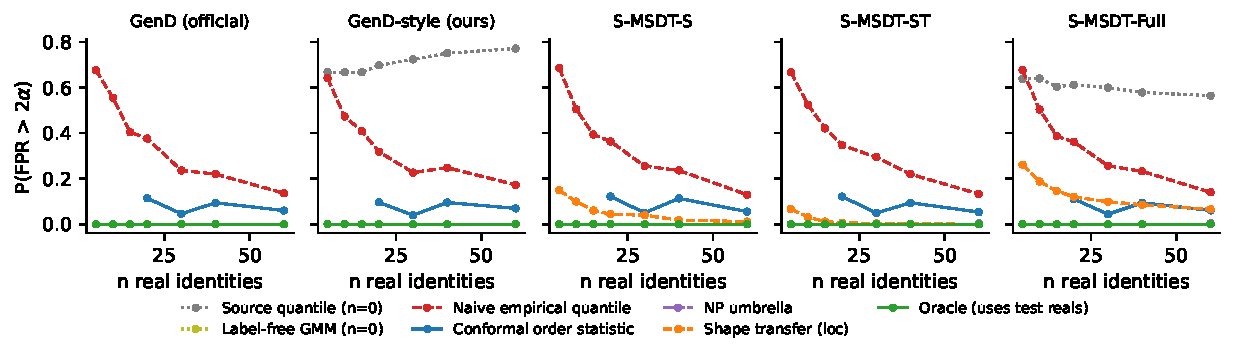
\includegraphics[width=\linewidth]{figures/confirm/fig4_real_shot_fail.pdf}
\caption{Frequency of draws whose audited FPR exceeds $2\alpha$ on FakeAVCeleb, as a function of $n$ ($\alpha=0.05$). Conformal values follow the Beta-Binomial prediction (about $0.12$ at $n=20$ and $0.05$ at $n=30$).}
\label{fig:appx_fail}
\end{figure}

\begin{figure}[h]
\centering
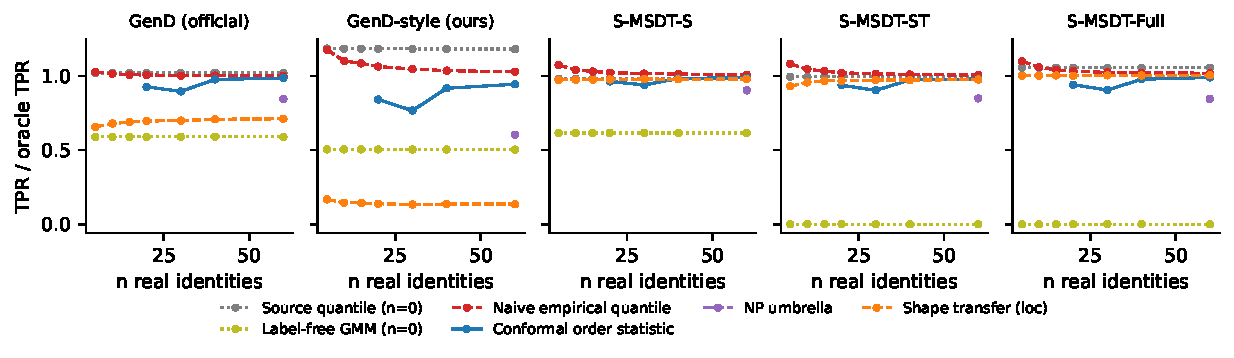
\includegraphics[width=\linewidth]{figures/confirm/fig3_real_shot_tpr.pdf}
\caption{TPR relative to the oracle threshold on FakeAVCeleb as a function of $n$ ($\alpha=0.05$). Ratios above 1 for the naive quantile reflect its higher false-alarm rate.}
\label{fig:appx_tpr}
\end{figure}

\section{Reproducibility}
\label{app:repro}
The supplementary archive contains the training configurations, data-split manifests and identity files, per-video score files for all 13 checkpoints and four test sets, calibration files, the evaluation and statistics code, the decision log, and \texttt{tools/paper\_tables.py}, which regenerates every table and Figure~\ref{fig:h8} from the committed results, and \texttt{tools/h8\_reseed\_check.py} for the post-hoc check of Table~\ref{tab:appx_h8_reseed}. The real-shot experiments use fixed random seeds (42 for the registered H8 run). Model weights will be released with the de-anonymized version.
